% !TEX root = ../my-thesis.tex
%
\selectlanguage{english}  
\chapter{\textcolor{ctcolormain}{Ecosystem services provided by \Qpw ("\textit{melojo}") forests}. A study case from Sierra Nevada (southern Spain)}\label{sec:es}

\mbox{}
\vfill
%{\color{ctcolormain}\textbf{Antonio J. Pérez-Luque}}; José V. Roces-Díaz \& Regino Zamora (In prep.)


\newpage

\paragraph{Abstract} \mbox{} \\
\Qp forests in Sierra Nevada have suffered intense anthropic pressures causing modifications in their structure and composition. Historically they were exploited in coppice for charcoal, firewood, or they were thinned and even burned to create grazing areas. However, the abandonment of traditional uses and exploitation since the middle of the last century has led to a decrease in anthropic pressure on these ecosystems. Paradoxically, some of these oak woodlands present a state of advanced degradation (stagnation of growth; scarce regeneration; etc), with stands with high densities and high biomass accumulation, increasing the fire risk. Taking into account this situation, and considering the vulnerability of this species to global change, it is necessary to search alternatives to the traditional uses of coppice management, particularly for those stands located in their rear edge (such us the oak woodlands of Sierra Nevada), due to their relevance for the species conservation. 
In this work we present a comprehensive review of the main ecosystem services provided by \Qpy focusing on oak woodlands located in Sierra Nevada mountain region.
\newpage

\section{Introduction}\label{sec:es:intro}

Mediterranean forests are subject to significant and simultaneous pressures \autocites{FAOPlanBleu2018StateMediterranean, DoblasMirandaetal2017ReviewCombination}, and climate change is expected to strongly affect to Mediterranean Region \autocite{GiorgiLionello2008ClimateChange, Penuelasetal2017ImpactsGlobal,Crameretal2018ClimateChange,Crameretal2020ClimateEnvironmental}, which is considered a hotspot for climate change \autocite{Giorgi2006ClimateChange}. The impacts of global change on Mediterranean forest ecosystems are altering the supply of ecosystem services \autocite{Lindneretal2010ClimateChange,Lindneretal2014ClimateChange,NoceSantini2018MediterraneanForest,Penuelasetal2017ImpactsGlobal,SerradaHierroetal2011ImpactosVulnerabilidad} particularly in mountainous regions, which have shown a high vulnerability to climate change \autocite{Schroteretal2005EcosystemService}. Notwithstanding, Mediterranean forests provide a wide range of ecosystem services (ES), and represent a great asset and opportunities for the future of the Mediterranean basin \autocite{Gauquelinetal2018MediterraneanForests, NoceSantini2018MediterraneanForest}. Hence, the importance of Mediterranean forests derives both from their current value in terms of area and goods and services, and from the role they are likely to play in the future \autocites{FAOPlanBleu2018StateMediterranean}.

Among the Mediterranean type forests, the oak woodlands are key ecosystems providing variety of ES \autocite{Maranonetal2020IberianOaks}. They provide regulating services such as climate regulation by their capacity to sequester carbon and therefore to mitigate the effects of climatic change; and contribute to regulation of the air, soil and water quality \autocite{Maranonetal2012EstadoTendencia}. Oak woodlands also provide several raw materials (provisioning services): cork, firewood, acorns \autocite{Bugalhoetal2011MediterraneanCork}. These forests also provide cultural ecosystems, such as recreational, aesthetic and spiritual \autocite{Lofetal2016ManagementOak}. In order to conserve the valuable goods and services provided for the benefit of the society and the environment, it is important to be aware of the potential of these forest, while respecting the carrying capacity these ecosystems can sustainability support. 


\subsubsection{The case of melojo woodlands (\Qpy) in the Western Mediterranean Region}\label{sec:es:intro-qp}
\Qpw (Pyrenean oak, \emph{melojo}) is a marcescent Mediterranean tree species widely distributed throughout southwestern France and the Iberian Peninsula reaching their southern limit in mountain areas of northern Morocco \autocites{Franco1990Quercus} (FIGURA 1). In the Iberian Peninsula, their forests occupy siliceous soils under meso-supramediterranean and mesotemperate areas and subhumid, humid, and hyperhumid ombroclimate \autocites{delaSernaetal2016MarcescentQuercus,Gavilanetal2018SclerophyllousDeciduous}. The rear-edge populations of this species are restricted to high-mountain areas where these populations persist as isolated nuclei with ecological conditions very different from those of the main distribution area \autocites{PerezLuqueetal2021EcologicalDiversity}. Sierra Nevada  mountains (37°N, 3°W, Spain) represent one of the southernmost European limit for this oak species (FIGURA 1B). In this mountain region, considered a glacial refuge for deciduous \emph{Quercus} species \autocite{Olaldeetal2002WhiteOaks}, there are eight Pyrenean oak patches (2400 ha) from 1100 to 2000 m \emph{a.s.l.}. They are the richest forest formation in vascular plant species of Sierra Nevada, containing several endemic and endangered plant species \autocite{Loriteetal2008PhytosociologicalReview}. They also harbor high levels of intraspecific genetic diversity \autocite{ValbuenaCarabanaGil2013GeneticResilience,ValbuenaCarabanaGil2017CentenaryCoppicing}. 

\Qp woodlands, like other forest ecosystems in Mediterranean area, have been subject to intense anthropogenic pressures over time \autocite{GarciaJimenez20099230Robledales}, resulting in a reduction of their extension and a modification of their floristic composition \autocites{Serradaetal1992CoppiceSystem,Gavilanetal2000EffectsDisturbance,PerezLuqueetal2021EcologicalDiversity} and structural patterns \autocites{Calvoetal1999PostfireSuccession,Tarregaetal2006ForestStructure}. Historically, \Qp woodlands have been exploited in coppices for firewood, charcoal, tannins, casca (\emph{i.e.} parts of the bark used to extract tannins), and other uses \autocites{RuizdelaTorre2006FloraMayor,SanchezPalomaresetal2008EstacionesEcologicas}. For instance, after the Spanish Civil war (since 1940's), some oak woodlands were massively cut down to use the firewood as fuel for automobiles (\emph{e.g.} Dehesa de San Jerónimo, Sierra Nevada)\autocite{Prieto1975BosquesSierra}. Forest management for \Qp coppices consisted of clear-cutting in rotation periods of 12-20 years, causing the profusion of shoots from the stool highly appreciated by livestock \autocite{Bravoetal2008SelviculturaMontes}. Thinning has also been carried out to create pastures with low densities of mature trees that provide acorns, firewood and large areas for grazing; and sometimes even burned to create grazing areas \autocites{HerreraCalvo2016UsoPastoral,Alvarezetal2009CambiosEstructura,ValbuenaCarabanaGil2017CentenaryCoppicing}. In fact, overgrazing in these formations have caused strong soil erosion loss, which was noticed by forest managers since the end of the 19th century \autocites{Laguna1872ComisionFlora}. In some areas, the strong anthropic pressure provoked the loss of the forest cover. For instance, in southern slopes of Sierra Nevada mountains, oak woodland forests were completely removed at the at the beginning of the 20th century, causing serious soil erosion problems, which led it to be considered the most torrential watershed in Spain \autocites{RomeroZurbano1909DivisionHidrologicoforestal}. All these anthropogenic processes have transformed the oak woodlands in a deep way that it is difficult to find stands that can be considered natural forests \autocites{RuizdelaTorre2006FloraMayor}. 

However, the abandonment of livestock and forestry traditional uses since the middle of the last century \autocites{MacDonaldetal2000AgriculturalAbandonment}, has caused a decrease in anthropogenic pressure on Mediterranean forest ecosystems \autocites{ValbuenaCarabanaetal2010HistoricalRecent}, being particularly important for mountain areas \autocites{JimenezOlivenciaetal2015MedioSiglo,JimenezOlivenciaetal2015EvolucionUsos,Piasetal2014ColonizationAbandoned}. Paradoxically, and considering this decrease in anthropogenic pressure, many of the \Qp oak stands present a state of advanced degradation, showing growth stagnation, lack of fruiting, and also sings of branch dieback  \autocites{Canellasetal2004GrowthResponse, Bravoetal2008SelviculturaMontes, ValbuenaCarabanaGil2014EfectosGestion, PiqueVericat2015EvolutionPerspectives, Piqueetal2018Spain}. Many stands also have high tree density that would increase the vulnerability to drought of these stands \autocite{McDowelletal2020PervasiveShifts}, and together with the accumulation of biomass and high horizontal continuity, would increase the risk of fire \autocites{Bravoetal2008SelviculturaMontes,GarciaJimenez20099230Robledales}. In addition, these problems may be aggravated in the current climate change context (increase in temperatures and higher incidence of extreme events such as droughts) \autocites{IPCC2013ClimateChange,Spinonietal2018WillDrought}, particularly considering the high vulnerability of this species to climate change \autocites{Benitoetal2011SimulatingPotential,GarciaValdesetal2013ChasingMoving,SanchezdeDiosetal2009PresentFuture,GeaIzquierdoetal2013GrowthProjections}, and especially for areas located in the rear edge of their distribution range such us Sierra Nevada mountain range.  

In view of this situation, the need to find for alternative uses for \Qp woodlands has been pointed out \autocites{MesonMontoya1985VegetacionForestal,SanMigueletal2012BosquesMatorrales}, and some management alternatives have been proposed \autocite[\emph{e.g.} sylvopastoral uses, see][]{HerreraCalvo2016UsoPastoral}. In this sense, the identification and characterization of the main ES becomes a crucial tool for providing a complete picture of the potential of these ecosystems, and to develop landscape planning and forest management strategies in a global change context \autocites{Piqueetal2018Spain}. 

Very little has been written about the ES provided by oak forests \autocites{Maranonetal2012OakTrees,Maranonetal2012EstadoTendencia,MorenoLlorcaetal2012MontanaMediterranea}. Some works have carried out a general valuation of the ES provided by the different \emph{Quercus} woodlands at regional and national scales \autocite{SanMigueletal2012BosquesMatorrales,Maranonetal2012EstadoTendencia,Sousaetal2020EcosystemServices}, and some studies provided temporal trend analysis of ES from an economic perspective \autocites[see][for an example for dehesas of California and Spain]{Caparrosetal2013EconomicsEcosystem}. However, to our knowledge, there is no comprehensive review of the ES provided by \Qp woodlands. 

The aim of this work is to carry out a review of the main ecosystem services provided by \Qp woodlands. We conduct a literature review to know the state of the art of the ES provided by these formations. Using the Sierra Nevada oak populations as study-case we explore more in depth the ES provided by this woodlands. For this purpose we combine expert knowledge and data coming from ecological monitoring programs and several research projects to quantify as far as possible the ecosystem services provided by this formation in Sierra Nevada. We hypothesized that the supply of ES are not equally distributed along the gradients within the Sierra Nevada, thus  we are also interested in how these ecosystem services are spatially distributed in this mountain region.

\section{Material and methods}\label{sec:es:mat}

To characterize the scientific literature that evaluate the ES of the Pyrenean oak woodlands, we performed a preliminary systematic search in the ISI Web of Knowledge (search date: October 2020). We compiled references published in indexed journals included in the Journal of Citation Reports (JCR), in English language, since 1970 to 2020, that evaluated indicators of ecosystem services in \Qp woodlands. First, we conducted a search for papers on the study species with the term \emph{"Quercus pyrenaica"} in the title, keywords or abstract, which produced 393 results. We applied a second criterion, to extract papers that analyzed possible services, including a broad list of terms (also in the title, keywords or abstract) related to ES (\tabref{tab:es:wos}). The combination of both produced 188 results. After reviewing their abstracts, we selected 60 papers that met the premise of evaluating ES in Pyrenean oak woodlands (\tabref{tab:es-review}). We omitted papers focused exclusively on descriptive aspects of these ecosystems (\emph{e.g.} floristic composition or ecosystem structure), their biodiversity (\emph{e.g.} species richness) which were not directly related to ecosystem service indicators. However, considering the local relevance of the \Qp oak woodlands in Sierra Nevada, we include biodiversity indicators in our analysis. 

\begin{table}[]
\caption{Search terms used in the literature review.}
\label{tab:es:wos}
\footnotesize
\begin{tabular}{>{\centering}p{11cm}l}
\toprule
\textbf{TOPIC (i.e. Title OR Keywords OR Abstract)} & \textbf{Results} \\ 
\toprule
\emph{"Quercus pyrenaica"} & 393 \\ \midrule
\emph{"ecosystem service*" OR "ecologic* process*" OR "ecologic*
function*" OR "provision*" OR "regulat*" OR "cultural" OR ``support*'' OR
"food" OR "mushroom*" OR "fruit*" OR "berry" OR "berries" OR
``cattle'' OR ``stock'' OR ``livestock'' OR ``sheep*'' OR ``goat*'' OR
``game'' OR ``hunt*'' OR ``wine'' OR "fresh water" OR "water supply" OR "drink* water" OR ``water
yield*'' OR ``firewood'' OR ``wood'' OR ``timber'' OR ``coal'' OR "climat* regulat*" OR "carbon sequest*" OR "carbon stock*" OR "carbon stor*" OR "soil fertilit*" OR "soil nutri*" OR "nutri* cycle*" OR "soil
carbon*" OR "organic carbon" OR "water regulat*" OR "soil water" OR "water cycle" OR "water stor*"
OR "water qualit*" OR "water depurat*" OR "water filtrat*" OR "water
clean*" OR ``snow regulat*'' OR ``snow storage'' OR "soil erosion" OR "soil protection" OR "erosion protection" OR
"erosion control" OR "soil loss" OR "water erosion" OR "landscape qualit*" OR "aesthetic*" OR "landscape value*" OR
"recreation*" OR "social percept*" OR ``spiritual value'' OR
``scientific knowledge''} & 188 \\
\bottomrule
\end{tabular}
\end{table}

For the classification and definition of ecosystem services, we adopted the CICES V5.1 (Common International Classification of Ecosystem Services) approach \autocites{HainesYoungPotschin2018CommonInternational}. This is an international effort to classify ecosystem services, which also has common points with other approaches such as the Millennium Ecosystem Assessment \autocite{MEA2005EcosystemsHuman}, and The Economics of Ecosystems and Biodiversity (TEEB) initiative \autocite{TEEB2010EconomicsEcosystems}. We have considered three categories of ecosystem services: provisioning, regulating and cultural. For each of these categories, different indicators related to the provision of specific ecosystem services were defined (\tabref{tab:es:data}). 

\begin{sidewaystable} 
\caption{Ecosystem Services (ES) indicators used in this study. For each indicator the ES category, references, units, and data source are indicated. (\emph{R}): regulation; (\emph{S}): provisioning and supporting; (\emph{C}): cultural. (*) extracted from the literature; (**) own calculations. (+) indicators with data for oak populations of Sierra Nevada.}\label{tab:es:data}
\centering
\scriptsize
\begin{adjustbox}{width=\linewidth}
\begin{threeparttable}
\begin{tabular}{>{\raggedleft}m{0.087\linewidth}>{\centering}m{0.108\linewidth}m{0.4\linewidth}>{\centering}m{0.102\linewidth}m{0.165\linewidth}m{0.071\linewidth}}
\textbf{Ecosystem Service} & \textbf{ES indicator used} & \textbf{Bibliographic References} & \textbf{Units} & \textbf{Data Source} & \textbf{Data for Sierra Nevada } \\ \toprule 
Experiential use of Landscape (C) & Number of photographies (*) & \autocite{MorenoLlorcaetal2020EvaluatingTourist} & Number of photographies & \autocite{RosCandeiraetal2020SocialMedia} & Yes (+) \\
Physical use of Landscape (C) & Wikiloc tracks (**) &  & Routes density; Total routes & Wikiloc & Yes (+) \\
Recreational (C) & Visitors numbers (**) &  & Visitor numbers & Sierra Nevada Natural and National Protected Area & Yes (+) \\
Scientific (C) & Research requests permisision (**) & \autocite{Zamoraetal2016GlobalChange} & Number of Research requests & Sierra Nevada Natural and National Protected Area & Yes (+) \\
Scientific (C) & Density of socio-ecological monitoring methodologies (**) & \autocite{Zamoraetal2016GlobalChange} & Density of monitoring methdologies & Sierra Nevada Natural and National Protected Area & Yes (+) \\
Symbolic (C) & Singular trees (*) & \autocites{IruritaFernandezetal2003ArbolesArboledas, SanchezGarciaetal2003ArbolesArboledas} &  & Andalusia Regional Goverment & Yes \\
Biodiversity (S) & Bird richness (**) & \autocites{BareaAzconetal2012PasseriformesOtras,PerezLuqueetal2016DatasetPasserine,ZamoraBareaAzcon2015LongTermChanges,PerezLuqueetal2021ManualGestion} & Species number & Sierra Nevada Global Change Observatory & Yes (+) \\
Biodiversity (S) & Fungal diversity (*) & \autocites{Ortegaetal2010MycorrhizalMacrofungi, MorenoArroyo2004InventarioMicologico} & Species number & Basic Mycological Inventory of Andalusia &  \\
Biodiversity (S) & Genetic diversity (*) & \autocites{ValbuenaCarabanaGil2013GeneticResilience,ValbuenaCarabanaGil2013ReduceAprovechamiento,ValbuenaCarabanaGil2014EfectosGestion,ValbuenaCarabanaGil2017CentenaryCoppicing} &  &  & Yes (+) \\
Biodiversity (S) & Microbial diversity (*) & \autocites{CoboDiaz2017,Lasaetal2019BacteriaEndosphere, Lasaetal2019MetabarcodingReveals} &  &  & Yes \\
Biodiversity (S) & Woody richness (*) & \autocite{PerezLuqueetal2014SinfonevadaDataset,Loriteetal2008PhytosociologicalReview} & Species number &  & Yes (+) \\
Food provision (S) & Wild mushrooms production (*) & \citet{RayaLopezetal2017MuestreosPara} & kg Fungi ha$^{-1}$ year$^{-1}$ & Plan CUSSTA (Plan for the Sustainable Use and Conservation of Mushrooms and Truffles in Andalusia) & Yes \\
Tanning (S) & Percentage of tannins (*) & \autocites{FernandezdeSimonetal2006ChemicalCharacterization,Doceetal2007EffectImmature,TornerOchoa1952CurtientesVegetales} & \% of tannis present at bark &  & \\ 
Timber (S) & Biomass increment & \autocite{PerezLuqueetal2021CarbonSequestration} & Mg ha$^{-1}$ year$^{-1}$ & Spanish National Forest Inventory & Yes \\
Wine Ageing (S) & Phenological compunds (*) & \autocites{Ramiloetal2017VolatileOrganic,Gallegoetal2012PhenolicCompounds, CadahiaFernandezdeSimon2004UtilizacionRoble,FernandezdeSimonetal2008VolatileCompounds,FernandezdeSimonetal2009VolatileCompounds, Gallego2013EstudioPotencial,MartinezGiletal2020EffectSize} &  &  &  \\
Climate Regulation (R) & Carbon sink (**) & \citet{PerezLuqueetal2021CarbonSequestration} & Mg CO$_2$ ha$^{-1}$ & LIDAR and Forest Inventories & Yes (+) \\
Climate Regulation (R) & Vegetation Index (NDVI, EVI) (*) & \autocites{Dionisioetal2012SatelliteBasedMonitoring,Alcaraz2016obsnev_ndvi,PerezLuque2015onto,Cazorlaetal2020RemoteSensingbased} &  & MODIS & Yes (+) \\
Climate Regulation (R) & Regulation of temperature (**) & \autocite{Zamoraetal2021UniendoMacro} &  & ClimaNevada & Yes \\
Control of erosion (R) & Soil erosion Control (*) & \autocites{MesonMontoya1985VegetacionForestal,Salomonetal2017GeneralFailure} &  &  &  \\
Soil Fertility Regulation (R) & Soil Organic Carbon (**) & \citet{Hengletal2017SoilGrids250mGlobal, Batjesetal2017WoSISProviding, Batjesetal2020StandardisedSoil} & Mg SOC ha$^{-1}$ & SoilGrid database & Yes (+) \\
\bottomrule
\end{tabular}
\end{threeparttable}
\end{adjustbox}
\end{sidewaystable}

For each of the ES reviewed, we performed a quantification for the Sierra Nevada oak woodland populations, as long as data were available. The values for the quantification were obtained both from the literature review and from several research datasets in combination with the expert criterion. For those ES with data availability, we performed a quantification for each of the oak population clusters identified in Sierra Nevada, \emph{i.e.} Northern (N), Northwestern (NW), and Southern (S)\autocite[ see][]{PerezLuqueetal2021EcologicalDiversity}. We compared differences in the supply of ES between the oak population clusters (\tabref{tab:es:oak-cluster}).

In the following section we present the most relevant results of the review of the main ES provided by \Qp woodlands. Where information is available, a special mention and/or analysis of existing data for Sierra Nevada has been added. 
 
\section{Ecosystem Services provided by \Qp woodlands}\label{sec:es:results}

The compilation of literature carried out has shown us those services that have been most frequently evaluated in works focused on \Qp woodlands (see \tabref{tab:es:wos}). Of the 60 papers selected in the literature review, provisioning services were the most frequently evaluated. Among them, the studies focused on investigating the effect of melojo wood in the wine production process stand out (\emph{n} = 26/60) \autocites[\emph{e.g.}][]{FernandezdeSimonetal2010CharacterizationVolatile,CastroVazquezetal2013EvaluationPortuguese}, since barrels are frequently built with the wood of this species. In addition, there are papers evaluating mushroom production \autocites[\emph{e.g.}][]{OriadeRuedaetal2010CouldArtificial}, or the effect of this species on livestock production \autocites[\emph{e.g.}][]{Nunezetal2012LivestockManagement}. There also were studies evaluating the production of wood or biomass for energy (\emph{n} = 6/60) \autocites[\emph{e.g.}][]{Mirandaetal2009EnergeticCharacterization}. Regarding regulation services, several studies evaluate the role of \Qp forests in soil quality and fertility (\emph{n} = 12/60), or their capacity for carbon sequestration and storage \autocites[\emph{n} = 12/60; \emph{e.g.}][]{Alvarezetal2014InfluenceTree}. There also a high proportion of studies on soil carbon \autocites[\emph{n} = 8/60; \emph{e.g.}][]{Fonsecaetal2019ImpactTree}. Finally, it should be noted that, applying the above-mentioned search criteria, no studies on the evaluation of cultural services in the \Qp ecosystems have been found.

\subsection{Regulating services}\label{sec:es:regulation}
\subsubsection{Soil climate regulation}\label{sec:es:regulation-soil}
The cover provided by woodlands is key to regulating soil temperature \autocite{Ellisonetal2017TreesForests}. Soil temperature is one of the main factors affecting seed germination, plant growth and development, being as important as air temperature, since it can limit root formation \autocites{AlvarezUriaKorner2007LowTemperature}. The marcescent feature of \Qp allows the accumulation of leaf litter layer on the ground during a part of the year. This accumulation can have positive effects on seedling establishment because it acts as a thermal insulator \autocites{Loydietal2014DistributionEffects}, helping to alleviate the damage effects of freezing on seeds \autocites{Loydietal2014DistributionEffects,CavenderBaresetal2005SummerWinter,EstesoMartinezGilPelegrin2004FrostResistance,Lofetal2019TammReview}. This buffer effect can also be important once germination starts, since negative temperatures can suspend the process and damage the radicle and epicotyl \autocites{AizenWoodcock1996EffectsAcorn}. However, negative effects on seed germination and establishment could prevail (\emph{e.g.}, pathogen proliferation; allelopathic effects) when litter accumulation exceeds a certain threshold \autocites{Loydietal2014DistributionEffects,XiongNilsson1999EffectsPlant}.

It has also been noticed the importance of the forest cover on the regulation of extremes temperatures registered during the summer period \autocites{DeFrenneetal2021ForestMicroclimates}. It is particularly important for melojo oaks woodland located at the warm rear-edge of their distribution. For instance, using microclimatic data from a sensor network deployed in an oak woodland located at southern slopes of Sierra Nevada, \citet{Zamoraetal2021UniendoMacro} found strong variations of the air and soil temperatures registered inside the \Qp forest compared with the registered on forest's open areas (\figref{fig:es:temp}). The soil temperatures varied up to 15ºC between microhabitats on a day of maximum temperatures during the summer period. This highlights the role of the oak tree vegetation on the regulation of the thermal environment \autocites{Niinemets2010ResponsesForest}. The oak forest cover provides a cooler environment, reducing potential evapotranspiration and alleviating the water stress to which these formations are subjected in summer \autocites{Zamoraetal2021UniendoMacro}.  

\begin{figure}[H]
    \centering
    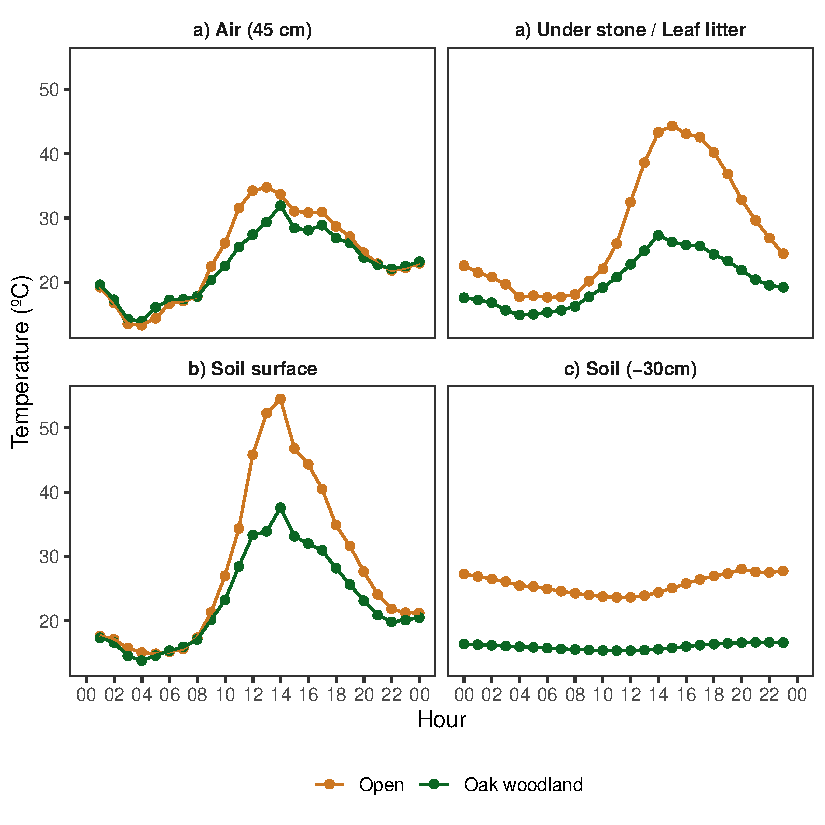
\includegraphics[width=\textwidth]{img/es/es-profiletemp.pdf}\caption{Hourly variation of the temperature on July 19, 2018 (hottest day of the 2018-2019 period in the "Robledal de Cáñar" oak woodland. \textbf{a)}. Variation in air temperature recorded at 45 cm in forest areas (green line) and in forest clearings (brown line). \textbf{b)}. Variation of the temperature for the covered soil (under stone; or under litter); anf of the temperature of the soil surface (\textbf{c}); and soil temperature at 30 cm depth (\textbf{c}). For each variable, the values recorded in the different habitats are compared: forest clearings (open) and forest areas (forest). Source: \autocite{Zamoraetal2021UniendoMacro}}\label{fig:es:temp}
\end{figure}

\subsubsection{Carbon sequestration}\label{sec:es:regulation-carbon}
Carbon sequestration is one of the most relevant ecosystem services provided by Mediterranean forests \autocites{Gauquelinetal2018MediterraneanForests,NoceSantini2018MediterraneanForest}. The carbon stock can be assumed as an indicator of the capacity of ecosystems to contribute to climate regulation due to their potential to influence the concentration of atmospheric CO$_2$ \autocites{Lauterbach2007AssessmentExisting,Luyssaertetal2008OldgrowthForests}. Mediterranean forests represent a carbon sink that is expected to increase in the coming decades \autocites{Canellasetal2017CarbonSequestration,PasalodosTatoetal2017EvaluationTree}, although recent studies have shown a ralentization of this increase \autocites[][]{RocesDiazetal2021TemporalChanges}.

Recently, a cartography of the biomass and carbon sequestration potential of \Qp woodlands of Sierra Nevada were generated \autocites{PerezLuqueetal2021CarbonSequestration} (see also chapter \ref{sec:carbon}). These authors, combining information from LIDAR (\emph{Light Detection And Ranging}) remote sensing with information from different forest inventories, estimated a total biomass (aboveground- and belowground-biomass) of 9.94 Tg (1 Tg = 10$^12$ g) in the \Qp forests of the Sierra Nevada, which represents a potential CO$_2$ sequestration of 17.33 Tg (1 Tg = 10$^12$ g). This highlights the importance of these forests in carbon sequestration, which represents a key ecosystem regulating service.

Spectral vegetation indices, \emph{e.g.} EVI and NDVI are frequently used to derive indicators of ecosystem functioning, such as the total annual carbon absorbed by vegetation, or the seasonality and phenology of carbon gain dynamics \autocites{Xiaoetal2019RemoteSensing,
AlcarazSeguraetal2009BaselineCharacterization,AlcarazSeguraetal2009UseDescriptors,Cazorlaetal2020RemoteSensingbased}. Some works have analyzed the evolution of the productivity of different ecosystems in Sierra Nevada using vegetation indices from MODIS satellite data \autocites{Dionisioetal2012SatelliteBasedMonitoring,Alcaraz2016obsnev_ndvi,PerezLuque2015onto,Cazorlaetal2020RemoteSensingbased}. The results of these works have revealed that melojo oak forests, despite their high seasonality, are the most productive ecosystems in Sierra Nevada for the period analyzed (2000-2017), highlighting their importance in carbon gain and therefore as carbon sinks. Likewise, the time series analysis showed a positive trend in productivity (EVI) for most Sierra Nevada oak forests, possibly related to the increase in temperature \autocite{PerezLuque2015onto}.

Soil organic carbon (\emph{SOC}), the main component of soil organic matter, is considered relevant for many soil processes. For example, SOC content correlates positively with soil fertility, playing a key role determining the physical, chemical and biological qualities of a soil \autocites{Victoriaetal2012BenefitsSoil}. There are different ecosystem services in which SOC is involved, among which regulation and provisioning services stand out \autocites{Francavigliaetal2018OrganicCarbon}. Despite, there are some studies that reported the amount of soil organic carbon in specific locations of the Sierra Nevada oak woodlands \autocites{CoboDiazetal2017TaxonomicFunctional,Lasaetal2019BacteriaEndosphere}, they prove insufficient to provide an approximated estimate of the total SOC content for those oak woodlands. There are, however, soil databases that providing estimates of the SOC content at a ecosystem level, such as the SoilGrid database (https://soilgrids.org/), which provides digital maps of different soil variables at a 250-m spatial resolution \autocites{Hengletal2017SoilGrids250mGlobal,Batjesetal2017WoSISProviding,Batjesetal2020StandardisedSoil}. For Sierra Nevada, those maps reported an average SOC content (mean SOC at 0-30 cm depth) of 51.8 Mg ha$^-1$ (20-80 Mg ha$^-1$) (\figref{fig:es:soc}), while the oak forests have a average SOC value of 53.5 Mg ha$^-1$ (45-67 Mg ha$^-1$), with southern oaks populations showing significantly higher values. 

\begin{figure}
    \centering
    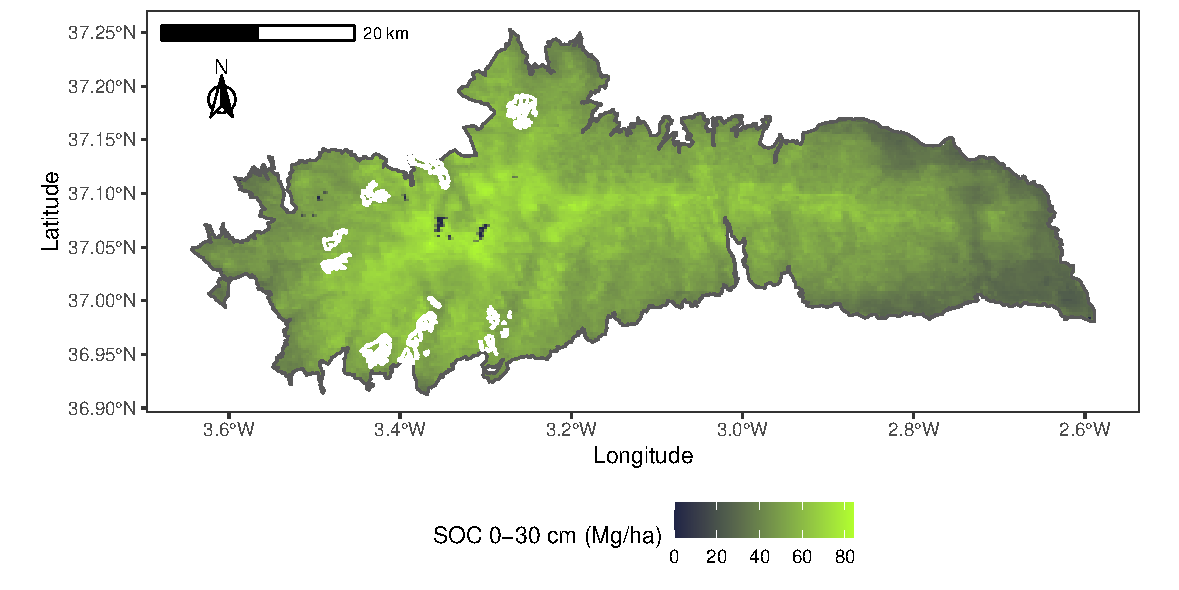
\includegraphics[width=\textwidth]{img/es/es-soc.pdf}\caption{Distribution of the Soil organic carbon in Sierra Nevada. Oak populations in white. Drawn with data from SoilGrid database \autocites[see][]{Hengletal2017SoilGrids250mGlobal}}\label{fig:es:soc}
\end{figure}

\subsubsection{Erosion control}\label{sec:es:regulation-erosion}
Forests have a key role in the reduction of the erosive rainfall impact on soil, so they provide an important regulating service \autocites{Zhongmingetal2010StratifiedVegetation,GarciaRuizetal2011MediterraneanWater}. The root system of \Qp consists of two well-differentiated types \autocites{Allue1995OrdenacionMasas}: \emph{(i)} the main root, characteristic of the genus, which allows for powerful anchoring to the soil; and \emph{(ii)} a layer of roots close to the soil surface and parallel to it, which could emit large number of shoots that form a dense network. Those root systems that help to maintain soil integrity by preserving landslides \autocites{MesonMontoya1985VegetacionForestal,Salomonetal2017GeneralFailure} (\figref{fig:es:roots}). In addition, the extraordinary regrowth capacity of \Qp, both of stump and roots, gives it functional advantages over other species, such as its response to disturbances (\emph{e.g.}, fires), particularly on sloping areas \autocites{RuizdelaTorre2006FloraMayor,ValbuenaCarabanaGil2017CentenaryCoppicing}. The profusion of resprouts provides an important ecosystem service of regulation, since the resprouts effectively maintain the soil in mountainous areas, reducing the impact of erosive processes and the soil loss  \autocites{MesonGarcia1984BasesEcologicas}.

\begin{figure}
    \centering
    \includegraphics[width=\textwidth]{img/es/es-roots.jpg}\caption{Structure of the complex root system of several specimens of \Qp. Picture from R. Salomón.}\label{fig:es:roots}
\end{figure}

\subsection{Supporting and provisioning services}\label{sec:es:provision}
\subsubsection{Biodiversity}\label{sec:es:provision-biodiversity}

\Qp forests in Sierra Nevada have high values of phytosociological uniqueness \autocites{Loriteetal2008PhytosociologicalReview}, which could be explained because they act as habitat providers for other relict species. In fact, the role of refugee of Sierra Nevada for this oak ecosystem \autocites{Breweretal2002SpreadDeciduous,Olaldeetal2002WhiteOaks,RodriguezSanchezetal2010TreeRange}, translates into a great diversity of plant species, being the forest formation with the greatest richness in Sierra Nevada, although it only represents 7\% of the forest area \autocites{PerezLuqueetal2014SinfonevadaDataset}. A key role of \Qp woodlands in Sierra Nevada is that they provides optimal conditions for the presence of several plant species cataloged under different threatened categories \autocites{Lorite2016UpdatedChecklist,Losaetal1986PaisajeVegetal,MelendoValle2000EstudioComparativo}, such as the hybrid mustard (\emph{Sorbus hybrida} L.) considered \emph{critically endangered} (CR), the \emph{endangered} (EN) goat willow (\emph{Salix caprea} L.), the holly (\emph{Ilex aquifolium} L.) and the yew (\emph{Taxus baccata} L.) considered \emph{vulnerable} (VU), and others with a lower level of threat (\emph{e.g.} \emph{near threat}, NT) (\emph{e.g.} the rowan, \emph{Sorbus aria} (L.) Crantz; or the maple \emph{Acer opalus} subsp. \emph{granatense} (Boiss.) Font Quer \& Rothm.). Many of these species are also considered relict species that find favorable microclimatic conditions in the melojo oak woodlands of Sierra Nevada, which make these ecosystems a refuge for those species \autocites{Blancaetal1998ThreatenedVascular,Lorite2016UpdatedChecklist,Losaetal1986PaisajeVegetal}. 

Birds community of \Qp forests of Sierra Nevada have been studied since 1980's \autocites{ZamoraCamacho1984EvolucionEstacional,ZamoraBareaAzcon2015LongTermChanges,BareaAzconetal2012PasseriformesOtras}. A total of 73 species of passerine bird species has been recorded within these oak forests \autocites{PerezLuqueetal2016DatasetPasserine}. Recent analysis shown differences in diversity between Sierra Nevada oak populations, with lower diversity values for southern oak populations than for northern-ones \autocites{PerezLuqueetal2021ManualGestion}. No differences was found for bird abundance, but a general decrease of several key species (\emph{Garrulus glandarius}) were recorded since 1980 \autocites{ZamoraBareaAzcon2015LongTermChanges}. 

Regarding the fungal community associated with this oak ecosystem, although there are no studies analyzing the composition for oak populations of Sierra Nevada, several works have shown the richness associated to this ecosystem at regional and national scales. Thus, an exhaustive review of the diversity of mycorrhizae-forming macromycetes in the \emph{Quercus} forests of the Iberian Peninsula recorded 174 fungi species in \Qp formations \autocites{Ortegaetal2010MycorrhizalMacrofungi}, of which 5 are included in the Red List of Fungi to be Protected in the Iberian Peninsula. At regional level, the Basic Mycological Inventory of Andalusia (IMBA, \emph{Inventario Micológico Básico de Andalucía}), reported 214 records belonging to 149 fungi taxa, inhabit in \Qp ecosystem \autocites{MorenoArroyo2004InventarioMicologico}. 

Another aspect to consider when analysing the biodiversity of the oak woodlands, is the presence of species using this trees. For instance, \emph{Quercus} species are key in the development of the biological cycle of some insects, such us the oak gall wasp (Hymenoptera: Cynipidae). The galls support species-rich, closed communities of inquilines and parasitoids that have become a model system in community ecology \autocites{Stoneetal2002PopulationBiology}. For instance, in melojo forests of Sierra Nevada have been recorded 30 species of cynipids (representing 21\% of the Iberian species) \autocites{NievesAldrey2013AvispasAgallas}. 

Several studies have analyzed the microbial diversity in the soils of some oak forests in the Sierra Nevada highlighting that the microbial community of this formation is dominated by a few very abundant taxa \autocites{CoboDiaz2017,Lasaetal2019BacteriaEndosphere, Lasaetal2019MetabarcodingReveals}. Finally, in relation to the genetic diversity, it has been traditionally assumed that continued coppicing of \Qp over centuries has led to a decline in the genetic diversity of the species, as a result of the strong inter-stem competition and the propagation of a limited number of genotypes 
\autocites{SanchezPalomaresetal2008EstacionesEcologicas,Bravoetal2008SelviculturaMontes}. However, several studies have pointed out the high diversity that these formations harbour \autocites{ValbuenaCarabanaGil2013GeneticResilience,ValbuenaCarabanaGil2013ReduceAprovechamiento,ValbuenaCarabanaGil2014EfectosGestion,ValbuenaCarabanaGil2017CentenaryCoppicing}. The high genetic diversity observed for the Sierra Nevada oak populations, highlights the importance of conserving the populations of this species which in this mountainous region are at the southern limit of their distribution, acting as a reservoir of genetic diversity. 

\subsubsection{Wine aging and tanning}\label{sec:es:provision-wine}
One of the characteristics of oak trees is their ability to emit volatile organic compounds (\emph{VOCs}), which in addition to giving the wines their characteristic flavor, act as an attractant for different insects. More than 50 volatile organic compounds belonging to 12 different chemical classes have been characterized in melojo oak \autocites{Ramiloetal2017VolatileOrganic}. The phenolic compounds produced by \Qp have similar chemical composition to those produced by the main oaks used in wine aging, such as American oak (\emph{Q. alba}) or French oak (\emph{Q. petraea}) \autocites{Gallegoetal2012PhenolicCompounds}. In fact, the results of comparative analysis between wines aged in barrels from these three oak species, have indicated that the wine aged in melojo oak presents oenological features similar to those of the other oaks, being also very positively valued by the wine tasters \autocites{CadahiaFernandezdeSimon2004UtilizacionRoble,FernandezdeSimonetal2008VolatileCompounds,FernandezdeSimonetal2009VolatileCompounds}. All these results highlight the potential use of wood and its derivatives from \Qp for wine aging, which had not been previously used in cooperage \autocites{Gallego2013EstudioPotencial,MartinezGiletal2020EffectSize} (\figref{fig:es:barrica}). 

The bark and leaves of the \Qp contain a great diversity and a high percentage of tannins (8\% of bark and 2-10\% of the wood corresponds to tannins) \autocites{FernandezdeSimonetal2006ChemicalCharacterization,Doceetal2007EffectImmature,TornerOchoa1952CurtientesVegetales}. For this reason, \Qp has been used as a tanning agent for leather, particularly the bark \autocites{TornerOchoa1952CurtientesVegetales}, since the bark of this oak species contains higher percentage of tannins than other \emph{Quercus} species (8\% versus 2-3\%) \autocites{TornerOchoa1952CurtientesVegetales}.

\begin{figure}
    \centering
    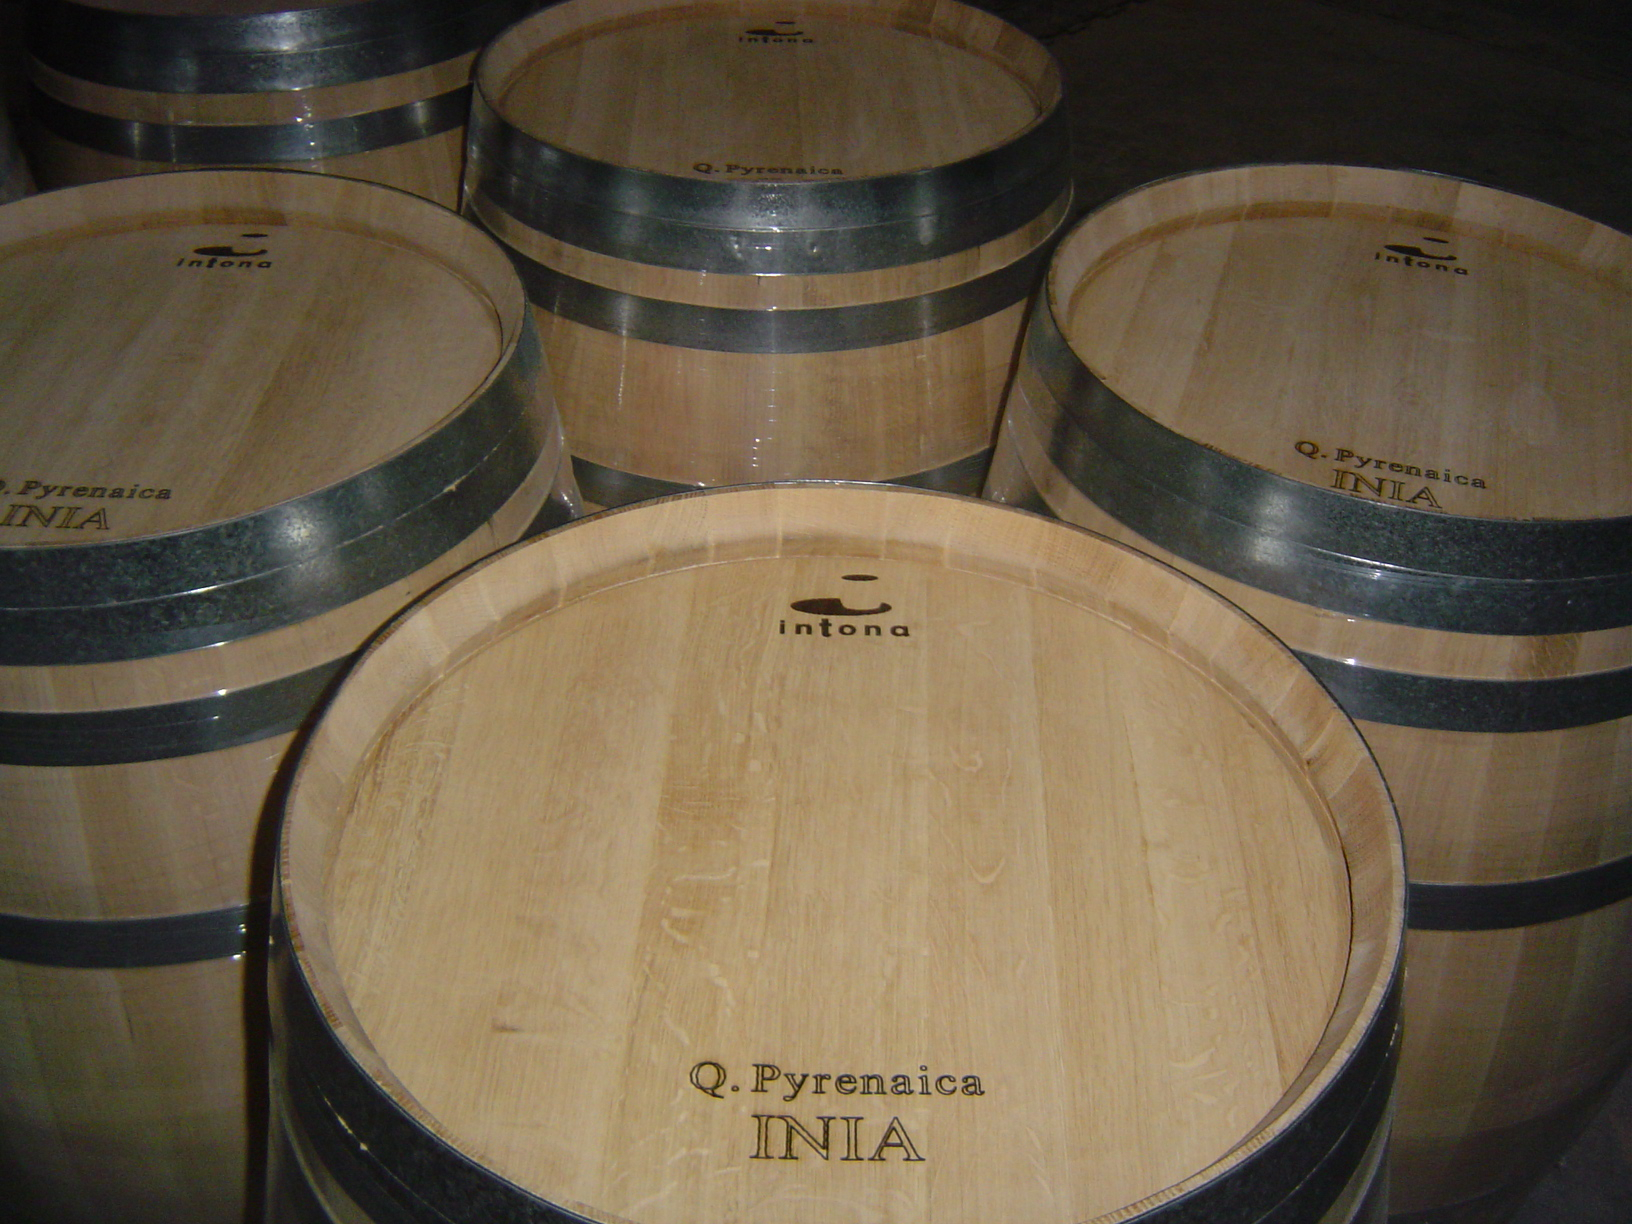
\includegraphics[height=6cm]{img/es/es-barrica.jpg}\caption{Melojo oak barrels for wine aging. Picture from Brigida Fernández de Simón}\label{fig:es:barrica}
\end{figure}

\subsubsection{Edible fungi}\label{sec:es:provision-fungi}
Mycological resources have high ecological, social, recreational and economic importance contributing to increasing the environmental asset value of the forests \autocites{MartinezPenaetal2015RentaAmbiental}. Mushroom picking has increased since 1980s and is becoming a important recreational activity. For European countries, 152 species belonging to 12 genera of wild mushrooms are commonly collected \autocites{Schulpetal2014WildFood}. Data on mushroom production and picking are scarce, scattered and heterogeneous. However, several initiatives have carried out preliminary assessment of mycological resources of forests, such as the RECAMAN initative in Andalusia ("Inncome and Capital of the Andalusian Mountains"; \emph{REnta and the CApital of the Montes de ANdalucía})\autocites{MartinezPenaetal2015RentaAmbiental}. Likewise, the "Plan CUSSTA" (\emph{Plan for the Sustainable Use and Conservation of Mushrooms and Truffles in Andalusia}) is carrying out periodic field sampling to determine the production of mushrooms in different forest formations in Andalusia \autocites{RayaLopezetal2017MuestreosPara}. Preliminary results for three years showed that in \Qp forests, the main marketable species are: \emph{Amanita caesarea} (3.63 \khy), \emph{Boletus aereus} (4.73 \khy), \emph{Cantharellus subpruinosus} (7.8 \khy), \emph{Hydnum rufescens} (0.23 \khy), \emph{Lepista nuda} (0.1 \khy), \emph{Macrolepiota procera} (0.41 \khy) and \emph{Russula cyanoxantha} (0.03 kg \khy). 

\begin{figure}
    \centering
    \includegraphics[height=6cm]{img/es/es-fungi.jpg}\caption{Collection of wild fungi in the surroundings of Robledal de Cáñar}\label{fig:es:fungi}
\end{figure}


\subsubsection{Timber production}\label{sec:es:provision-timber}
The wood of \Qp has not been appreciated as much as that of other oaks, although it has been used to obtain firewood directly or for charcoal production \autocites{MontoyaMeson1979SituacionActual}. For instance, some of the oak populations of Sierra Nevada have been intensely exploited to obtain wood \autocites[\emph{e.g.} Robledal de Cáñar, Alpujarras,][]{ValbuenaCarabanaGil2013GeneticResilience,MorenoLlorca2016}. In addition, other uses of timber have been documented in this mountain range, such as its use in mining in the northernwestern oak woodlands of Sierra Nevada \autocites{Titos1990}, where the timber of this species was used for mine tunnels and furnaces, and also as firewood to melt the mineral \autocites{Titos1990}. All these heavy exploitation of timber provoked an alteration in the oak forests structure \autocite{PerezLuqueetal2020LanduseLegacies}. Notwithstanding, since the 1970s, anthropogenic pressure on the forests has been reduced, which lead an increase of tree density, and also in the basal area and tree size \autocite{GonzalezDiazetal2020BosquesEspanoles}. This general pattern, observed for the forest of Iberian Peninsula \autocite{Astigarragaetal2020EvidenceNon,GonzalezDiazetal2020BosquesEspanoles}, has been also confirmed for Pyrenean oak forest. Thus, using data from second and third Spanish National Forest Inventory \autocites{VillaescusaDiaz1998SegundoInventario,Villanueva2005TercerInventario}, the temporal variation on tree biomass of the \Qp forests was assessed \autocites{PerezLuqueetal2021CarbonSequestration} (see also chapter \ref{sec:carbon}). The results shown a total increase of 19 172 \mgha between the two national forest inventories, with most of the inventories plot showing an increase pattern (89\%). This increase could be considered an asset for local populations around the oak woodlands, who could use the forest for firewood extraction.

\subsection{Cultural services}\label{sec:es:cultural}
\subsubsection{Recreational values}\label{sec:es:cultural-recreation}
Nature recreation represents a valuable ecosystem service that has a substantial economic value and contributes considerably to income and employment of local communities \autocites{Schagneretal2017MonitoringRecreation}. Monitoring visitors to natural areas have been used to estimate the recreational values provided by several ecosystems \autocites{Andersenetal2014MonitoringVisitors,Schagneretal2017MonitoringRecreation}. We used data from pyroelectric sensors located in several areas of the Sierra Nevada Protected Area to monitor visitors to this mountain range. We selected data located on two singular oak woodlands of Sierra Nevada for which data are available: Dehesa del Camarate, popularly known as \emph{"Bosque Encantado"} (Enchanted Forests), and Vereda de la Estrella. We analyzed the annual profile of the visits (October 2018 to 2019), and compared the visits in the two oak woodlands with total visitors registered for all sensors installed in this mountain region (\emph{n} = 14). Preliminary results showed that those two oak woodlands have a high number of visits, particularly during autumn season, when they represent almost the total number of visits (\figref{fig:es:visitorsprofile}). 

\begin{figure}
    \centering
    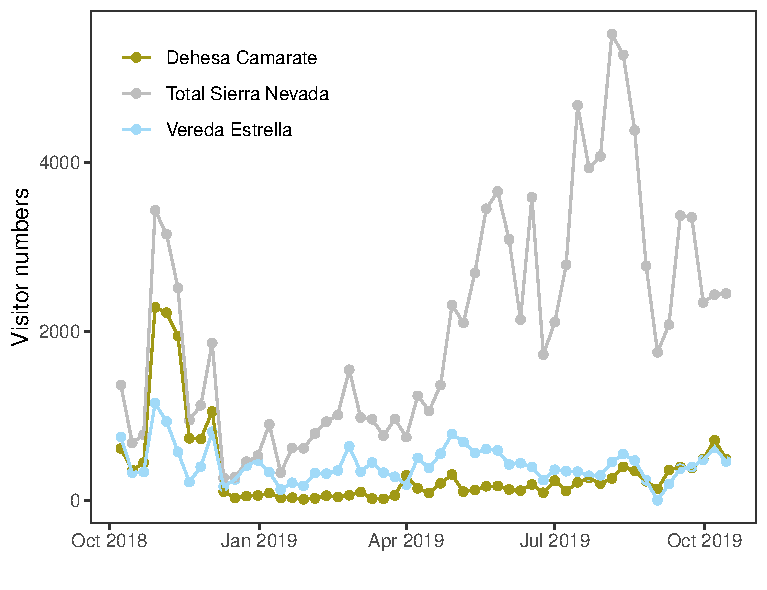
\includegraphics[width=0.9\textwidth]{img/es/es-visitorsprofile.pdf}\caption{Evolution of the visitors numbers in two oak woodlands, \emph{Dehesa del Camarate} (green), and \emph{Vereda de la Estrella} (blue), comparing with the total of Sierra Nevada (gray). Data come from automatic counters (pyroelectric sensors) located at different points in the Sierra Nevada.}\label{fig:es:visitorsprofile}
\end{figure}

\subsubsection{Recreational sports activities}\label{sec:es:cultural-sports}
One way to analyze the physical use of the landscape, and therefore its value as a provider of a cultural ecosystem service, consists of estimating the recreational activities performed in nature \autocites[\emph{e.g.}][]{RocesDiazetal2018AssessingDistribution}. We used the density of routes (hiking, biking, running and other types of outdoor activities) existing in the Wikiloc portal (www.wikiloc.com) (data query in January 2020) for all the municipalities belonging to the Sierra Nevada Natural Protected Area. For each municipality, the total number of routes, and the density (number of routes / surface area of the municipality in ha) were calculated (\tabref{tab:es:wikiloc}). Each of the oak populations of Sierra Nevada were assigned to the municipalities in which they are present. Of the 47998 routes obtained for the Sierra Nevada mountain region, 49.94\% were in the 14 municipalities where oak woodland are present (\figref{fig:es:wikiloc}). The density of routes in these municipalities ranged from 5.24 - 41.8 routes km$^{-2}$ (\tabref{tab:es:wikiloc}) being for most of them much higher than the average density of routes of the Sierra Nevada municipalities (17.88 routes km$^{-2}$). In absolute terms, the municipalities of the Alpujarra have the highest number of routes.

\begin{table}[]
\caption{Wikilock routes density (routes km$^{-2}$), and routes total numbers, for the municipalities of Sierra Nevada where Pyrenean oak woodland are located}
\label{tab:es:wikiloc}
\resizebox{\textwidth}{!}{%
\begin{tabular}{lllllllll}
\toprule
Oak population & CAM & GEN & MON & DIL & DUR & CAN & POQ & TRE \\ \midrule
Tracks density & 18.51 & 13.79 & 35.63 & 14.22 & 24.36 & 32.48 & 52.77 & 29.89 \\
Total tracks & 1170 & 3290 & 3170 & 1140 & 1870 & 555 & 1491 & 1908 \\ \bottomrule
\end{tabular}%
}
\end{table}

\begin{figure}
    \centering
    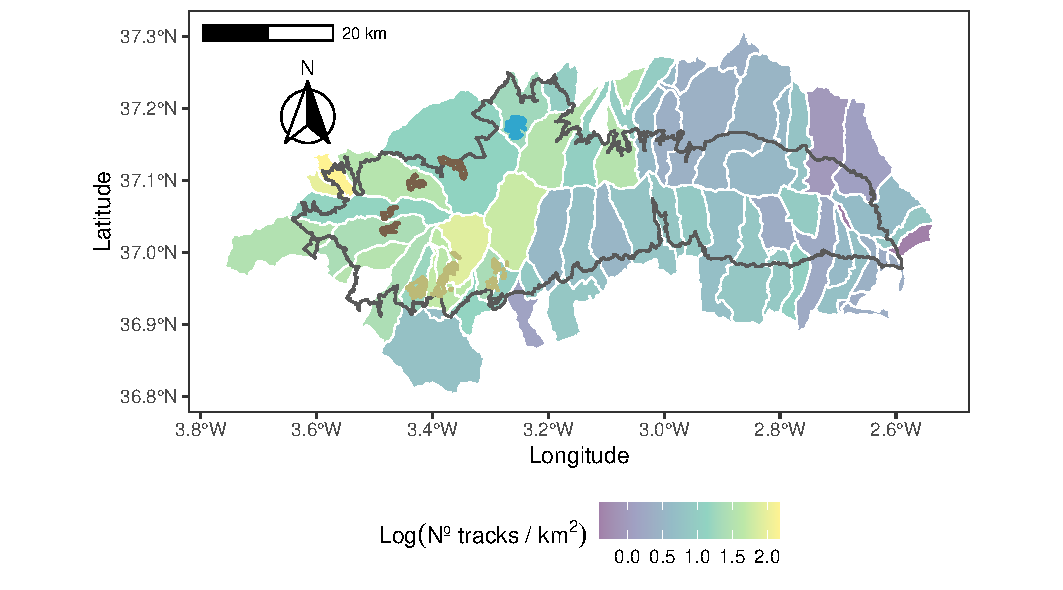
\includegraphics[width=\textwidth]{img/es/es-wikiloc.pdf}\caption{Density of Wikiloc routes for the municipalities of Sierra Nevada (Data from January 2020). Data are shown in Logarithmic scale.}\label{fig:es:wikiloc}
\end{figure}

\subsubsection{Scientific knowledge}\label{sec:es:cultural-scientific} 
To determine the importance of oak woodlands in the supply of the ES scientific knowledge, we used two indicators related to research activities. First, we explore the spatial location of research activities conducted in Sierra Nevada during the period 2009-2013 \autocites{Zamoraetal2017MonitoringGlobal}. For this purpose, a database compiling the research authorization documents for the Sierra Nevada Protected Area, was used to generate a density map with the \emph{hotspots} areas of research activities for Sierra Nevada mountain area. Then we extracted the information for the oak populations. Most of the research authorizations are concentrated in the western side of the Sierra Nevada (\figref{fig:es:scientific}b) particularly in the high summits area. The mean values of research permissions for oak woodlands in the period studied was 3.03 ± 0.06, with Genil and Cáñar oak populations (northwestern and southern oak populations respectively), contain the high concentration of research requests (\figref{fig:es:scientific}b). 
Secondly, we explored a density map of sampling protocols deployed in the Sierra Nevada \autocites{Zamoraetal2017MonitoringGlobal} using data from Sierra Nevada Global Change Observatory \autocites{Zamoraetal2016GlobalChange}. All the social-ecological monitoring protocols within this initiative were geolocated to generate a concentration map of sampling protocols by applying geostatistical hotspot detection techniques (Kernel density estimation) \autocites{Zamoraetal2016GlobalChange} (\figref{fig:es:scientific}a). The results show that the melojo oak woodlands are located in areas of high density of scientific activity (both sampling protocol density and research requested areas) in comparison with the other forest ecosystems of the Sierra Nevada.

\begin{figure}
    \centering
    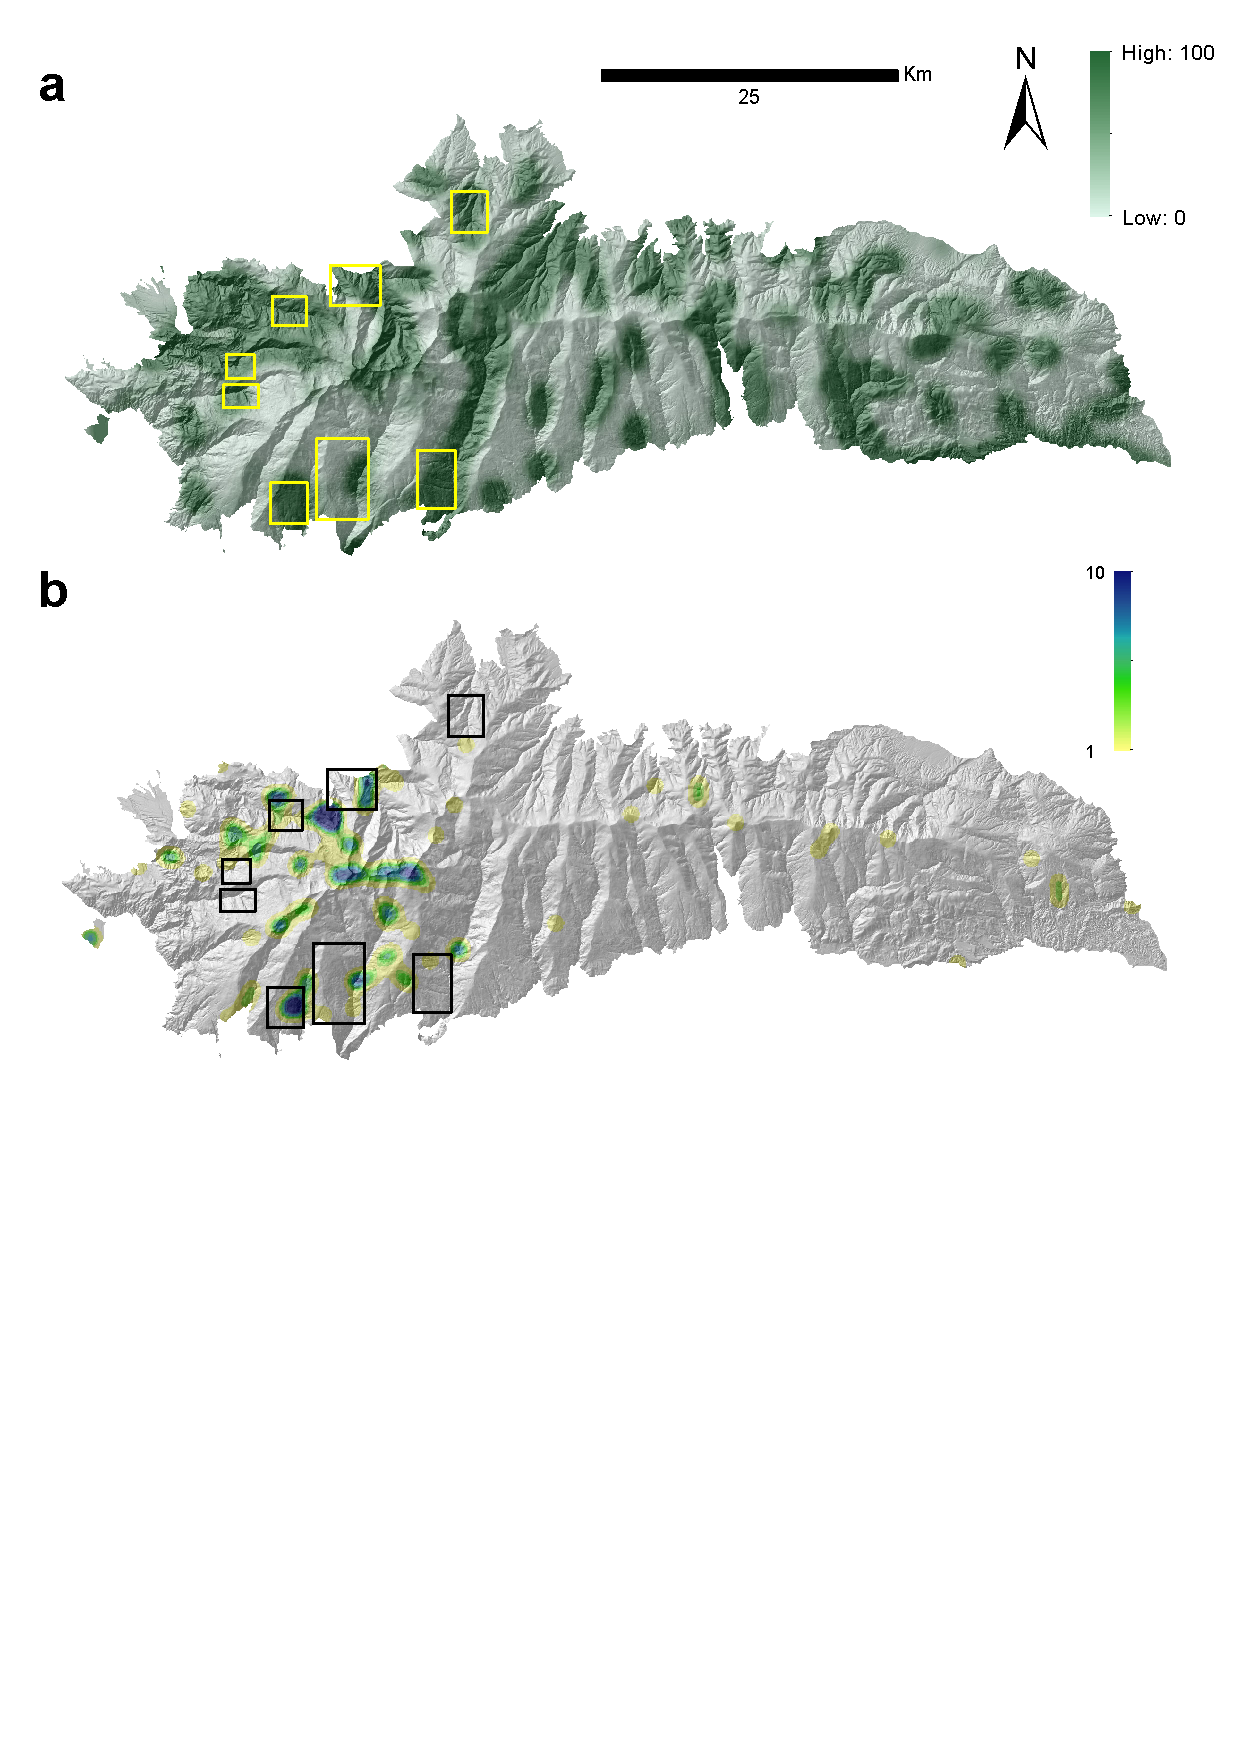
\includegraphics[width=\textwidth]{img/es/es-scientific.pdf}
    \caption{Spatial localization of the research authorizations (Number of research authorizations) performed in Sierra Nevada in the period 2009-2015 (\textbf{a}); and map of density (scaled density) of socioecological monitoring protocols carried out in Sierra Nevada since 2008 (\textbf{b}). For both maps the spatial bounding boxes of each oak population are shown. Drawn from \autocites{Zamoraetal2017MonitoringGlobal,Zamoraetal2016GlobalChange}}\label{fig:es:scientific}
\end{figure}

\subsubsection{Aesthetic values}\label{sec:es:cultural-aesthetic} 
Using data from the Flickr platform (www.flickr.com), \citet{MorenoLlorcaetal2020EvaluatingTourist} assessed some of the cultural services offered in Sierra Nevada. Of the total of 778 photographs analyzed, 18 are geolocated in oak woodlands (\figref{fig:es:flicker}). This value is low with respect to the total number of photographs analyzed, mainly due to the fact that the highest density of photos in the dataset analyzed is located around the ski resort and village areas (mainly the Alpujarras) \autocites{RosCandeiraetal2020SocialMedia}. Likewise, when we explore the various ecosystems in which the photos are located, we observe a higher concentration of photos in the high mountain areas. If we explore forest ecosystems (\emph{i.e.} native pine, holm oak, Pyrenean oak forests, and pine plantations), the photos taken in Pyrenean oak forests represent 32\% of the total.

\subsubsection{Singular trees}\label{sec:es:cultural-trees} 
Singular, large and/or monumental trees perform key ecological functions \autocites[\emph{e.g.} nutrient cycling; support complex assemblages of species,][]{Zapponietal2017RoleMonumental}. They have important impacts on the distribution and abundance of many other entities, from water and nutrients to whole organisms (fungi, other plants and numerous animal species) \autocites{LindenmayerLaurance2017EcologyDistribution}. Furthermore, they are creditors of natural value \emph{perse} \autocites{Asciutoetal2016MonumentalTrees}, and are considered part of a social realm, providing numerous socio-cultural benefits to society \autocites{BlicharskaMikusinski2014IncorporatingSocial,MoyaMoya2013MonumentalTrees}. Singular trees provide humans with aesthetic, symbolic, religious and historical values, as well as concrete tangible benefits, such as leaves, branches or nuts \autocites{BlicharskaMikusinski2014IncorporatingSocial}. They can be considered as single trees by their dasometric (height, diameter at breast height), age, and socio-cultural characteristics (\emph{e.g.} surrounding landscape, local myths, legends and traditions, witnessing historical events), so their conservation could contribute to the protection of both ecological and also social values \autocites{BlicharskaMikusinski2014IncorporatingSocial}. 

\begin{figure}
    \centering
    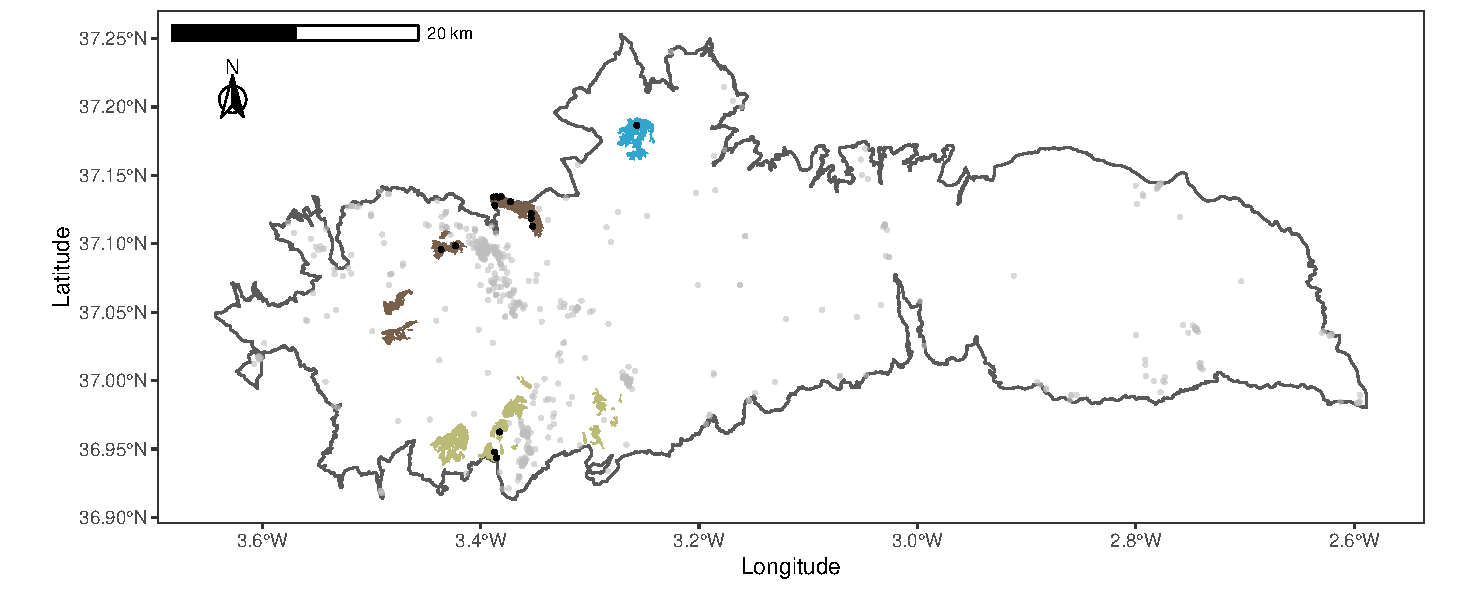
\includegraphics[width=\textwidth]{img/es/es-flicker.pdf}\caption{Location of photos taken in Sierra Nevada uploaded to the Flickr platform (\emph{n} = 778). Black dots indicate photos located in oak woodland. Drawn with data from \citet{RosCandeiraetal2020SocialMedia}. Oak woodland populations are shown. Colors correspond to northern (\emph{blue}), northwestern (\emph{brown}) and southern cluster's of oak woodlands identified for Sierra Nevada \autocite{PerezLuqueetal2021EcologicalDiversity}.  
}\label{fig:es:flicker}
\end{figure}
 
There are several individuals of \Qp in Sierra Nevada considered singular and/or monumental because of their extraordinary dimensions \autocite{IruritaFernandezetal2003ArbolesArboledas}, reaching tree heights of up to 19.5 meters and base perimeter of 6.7 meters. They are located in Busquístar (Alpujarras, southern slopes of Sierra Nevada). There are also other species singular trees located in the surroundings of some meolojo oak populations that add an ecosystem value to these oak populations, since these specimens are visited by hikers. For instance, in the Vereda de la Estrella (Güejar Sierra) there are majestic specimens of chestnut (\emph{Castanea sativa}), with a famous tree known as "El Abuelo" ("The grandpa") standing more than 20 m high and with a perimeter at the base of 10.7 m. Likewise, there are some oak woodlands in Sierra Nevada that shelter specimens and/or singular populations of other species. For instance, the Abedular del Barranco de los Alisos, located in the Dúrcal oak woodland \autocites{MartinezLabargaetal1990AbedularRelictico}. It is a small grove of about 300 individuals of birch (\emph{Betula pendula} subsp. \emph{fontqueri}) with an average height of 12 m. Other examples are the grove of birch trees located at the "Barranco de los Alisos", in the Dúrcal melojo population; or the Aliseda de la Cueva del Santo, where there are more than 100 alders (\emph{Alnus glutinosa}) accompanied by melojo oak and chestnut trees. In Andalusia region, there are also other melojo stands catalogued as singular, such as those located in the Sierra del Aljibe, whose specimens do not stand out for their dimensions but their location is unique and of great interest, representing a southern limit of distribution of the species \autocite{SanchezGarciaetal2003ArbolesArboledas}. 

\subsection{Spatial pattern for Ecosystem Services of Sierra Nevada}\label{sec:es:spatial} 

The quantification of some ES provided by melojo oak populations in Sierra Nevada, allows us to compare the supply of ES among those populations and to describe what ES category predominate for each of the oak population cluster’s in this mountain region. Regarding the regulation services evaluated, we observed that the southern populations have higher values for carbon sequestration potential, mean EVI and soil organic carbon than for the other clusters (\figref{fig:es:oak-compare}), despite the expected greater vulnerability due to their location in the southernmost areas of Sierra Nevada. Those results are in line with previously studies highlighted higher resilience values to disturbance of the southern oak woodlands \autocites{PerezLuqueetal2020LanduseLegacies}. For cultural ecosystem services, the NW populations present high values for sports activities, number of visitors, and density of sampling protocols (scientific value). Finally, for provisioning and support services we observed a variable pattern depending on the ecosystem service evaluated. 

\begin{figure}
    \centering
    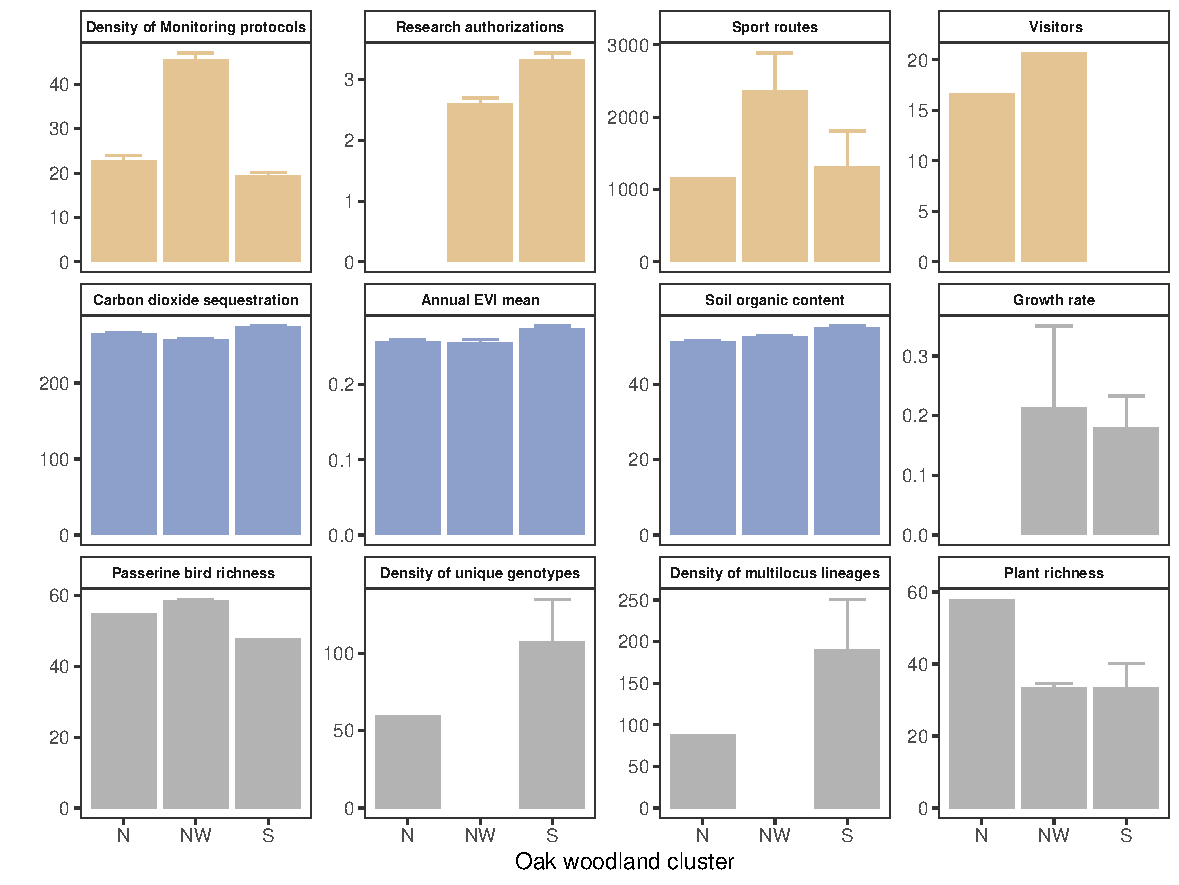
\includegraphics[width=\textwidth]{img/es/es-plotSN.pdf}\caption{Comparison of ecosystem services (cultural: yellow; regulation: blue; supporting: gray) for oak populations cluster identified in Sierra Nevada. See Table \tabref{tab:es:oak-cluster} for a detailed description 
}\label{fig:es:oak-compare}
\end{figure}

\section{Concluding remarks}\label{sec:es:concluding} 
In this work we combined a literature review with expert criterion to identify the ecosystem services provide by \Qp woodlands The literature review revealed the existence of a large number of works related to wine ageing, highlighting the potential of this species for wine production (\tabref{tab:es:wos}). It is striking that no work has been found in our literature review that evaluates cultural services in this woodland forests. However, this pattern changes when the ecosystem services are analyzed in more detail as in our case study. Thus, the combination of expert criteria with data at a more local scale allowed us to highlight the existence of a large number of cultural ecosystem services provided by \Qp woodlands. 
Our review of local data has allowed us to quantify many of the ES provided by melojo oak woodlands, which on the one hand highlights the values of these forest formations, and on the other hand, provides to natural resource managers with more information and tools to help them in the decision-making process. Incorporating information on ecosystem services can help in the planning of forestry actions for those oak woodlands. Our study also adds some interesting insights for the study of ES provided by forests. For instance, we observed a highly temporal pattern of some ES, such as the recreational values. Some melojo woodlands of Sierra Nevada concentrate a large part of the visitors recorded in the Sierra Nevada Natural Area (\figref{fig:es:visitorsprofile}) during a specific time period. This highlighting the needing to consider the temporal pattern of the ES evaluated, and to pay attention to the pressure that these ecosystems may be suffering temporarily due to the high number of visitors they receive. Therefore, from a natural resource management point of view,  it is not only necessary to analyse the ES provided by an ecosystem, but also we would consider the spatio-temporal pattern of the ES supply. In this sense, it would be interesting to carry out detailed studies to provide managers with a comprehensive assessment of the possible impacts of visitors.

\begin{sidewaystable}
\caption{Quantification of several Ecosystem Services (ES) for Sierra Nevada oak population clusters \autocites[see][]{PerezLuqueetal2021EcologicalDiversity}. N: Northern populations, NW: Northwestern populations; S: Southern populations.}\label{tab:es:oak-cluster}
\centering
\scriptsize
\resizebox{\linewidth}{!}{%
\begin{tabular}{>{\hspace{0pt}}m{0.14\linewidth}>{\hspace{0pt}}m{0.402\linewidth}>{\hspace{0pt}}m{0.158\linewidth}>{\centering\hspace{0pt}}m{0.075\linewidth}>{\centering\hspace{0pt}}m{0.085\linewidth}>{\centering\arraybackslash\hspace{0pt}}m{0.077\linewidth}} 
\toprule
\textbf{ES Indicator} & \textbf{Definition} & \textbf{Units} & \textbf{N} & \textbf{NW} & \textbf{S} \\
Plant richness & Mean richness of plant species recorded in forest invetories & Species number & 58 & 33.5 ± 1.04 & 33.5 ± 6.69 \\
Passerine bird richness & Mean richness of passerine birds recorded at bird censuses on oak woodlands & Species number & 55 & 58.5 ± 0.5 & 48 \\
Genetic diversity & Density of genotypes represented by one stem (unique genotypes, GU) per hecatera & Genotypes Uniques ha$^{-1}$ & 60 &  & 107.5 ± 27.5 \\
Genetic diversity & Density of multilocus lineages (MLL) per hectarea & Multiloculs Lineages ha$^{-1}$ & 89 &  & 191 ± 60 \\
Biomass increment & Increment of Biomass amount (Growth rate) between two National Forest Inventories (SNFI2 and SNFI3) & Mg Biomass ha$^{-1}$ year$^{-1}$  &  & 0.214 ± 0.136 & 0.18 ± 0.053 \\
Recreational values & Percentage of visits (visits registered in the oak woodland / total visits registered in Sierra Nevada) & \% & 16.69 & 20.68 &  \\
Sport activities (total routes) & Mean of total routes registered at Wikilock in the Municipalities where oak woodlands are located & Sport activites & 1170 & 2367.5 ± 520.36 & 1318 ± 489.95 \\
Scientific research authorizations & Average values of the Kerneld Density Estimate of the research permissions & Number of autorization research &  & 2.61 ± 0.09 & 3.34 ± 0.1 \\
Scientific sampling density & Average of Normalized Kernel Density Estimation of the Density of Monitoring methodologies & scaled value (0-100) & 22.94 ± 1.07 & 45.56 ± 1.52 & 19.57 ± 0.59 \\
EVI mean & Average of annual EVI mean for all pixels covering oak woodlands populations (period 2000-2018) &  & 0.257 ± 0.003 & 0.256 ± 0.004 & 0.275 ± 0.003 \\
Potential Carbon sequestration & Aveage values of the CO$_2$ potential sequestration & Mg CO$_2$ ha$^{-1}$ & 265.07 ± 1.41 & 256.72 ± 1.05 & 273.91 ± 0.93 \\
SOC & Average values of the mean Soil organic content at a 0-30 cm depth & Mg SOC ha$^{-1}$ & 51.27 ± 0.29 & 52.59 ± 0.34 & 55.11 ± 0.33 \\
\bottomrule
\end{tabular}
}
\end{sidewaystable}